% Modified by ARR to show two pictues in the same page
% changed page size; no page number
% use figure for each tizkz

% Unit circle
% Author: The Author
% What this does
\documentclass{article}
\usepackage[paperheight=6in,paperwidth=6in]{geometry}
\usepackage{tikz}


\usetikzlibrary{mindmap}

\pagestyle{empty}  % no page number

%\usepackage[top=1in,bottom=1in,right=1in,left=1in]{geometry} % margins

\begin{document}

\begin{figure}
	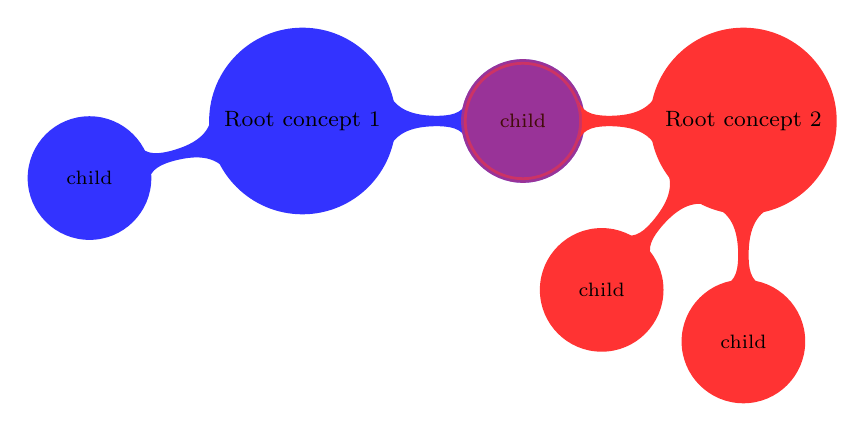
\begin{tikzpicture}[small mindmap,concept color=blue!80]
	\node [concept] {Root concept 1}
	child[clockwise from=0] {node[concept] {child}}
	child[clockwise from=270] {node[concept] {child}};
	\begin{scope}[concept color=red!80]
	\node [concept] at (5.6,0) {Root concept 2}
	child[clockwise from=180] {node[concept,opacity=0.5] {child}}
	child[grow=230 ] {node[concept] {child}}
	child[grow=270 ] {node[concept] {child}};
	\end{scope}
	\end{tikzpicture} 
\end{figure}

\begin{figure}
	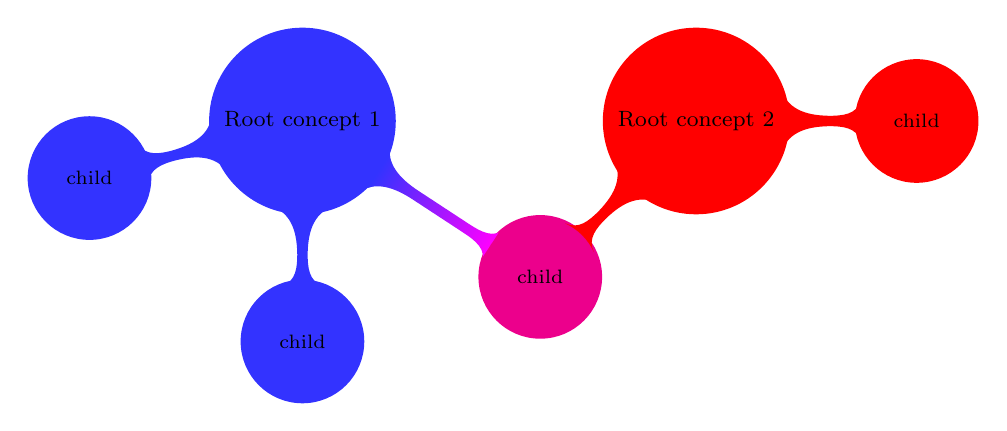
\begin{tikzpicture}[small mindmap,concept color=blue!80]
	\node (n1) [concept] {Root concept 1}
	child[clockwise from=270] {node[concept] {child}}
	child[clockwise from=270] {node[concept] {child}};
	\begin{scope}[concept color=red]
	\node (n2) [concept] at (5,0) {Root concept 2}
	child[clockwise from=225] {node[concept, concept color=magenta] (c1) {child}}
	child[grow=0 ] {node[concept] {child}};
	\end{scope}
	
	\path (n1) to [circle connection bar switch color=from (blue!80) to (magenta)] (c1);
	\end{tikzpicture} 
\end{figure}

\end{document}
